\newcounter{espPins}
\def\espWidth{4}
\def\espHeight{10}
\def\espScrewThickness{0.125}
\def\espPinHoleThickness{0.07}
\def\espButtonThickness{0.1}

\ctikzsubcircuitdef{spicesp}{
    vin%
} {
    coordinate (#1-start)
    node (#1) [inner sep = 0pt, anchor = center] {
        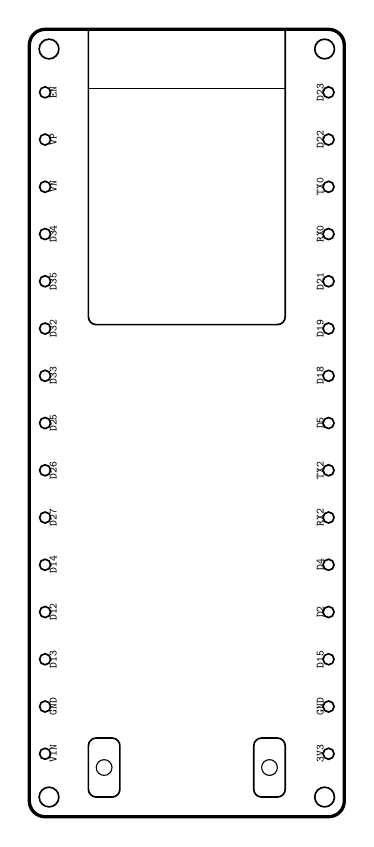
\begin{tikzpicture}
            \setcounter{espPins}{0}
            \draw [rounded corners = 2mm, very thick]
            (0,0) coordinate (origin)
            (origin) rectangle ++(\espWidth,-\espHeight)
            %% ++(-\espWidth,0) coordinate (some)
            ;
            \draw [semithick] (origin) ++(0.25,-0.25) circle (\espScrewThickness) ;
            \draw [semithick] (origin) ++(\espWidth,0) ++(-0.25,-0.25) circle (\espScrewThickness) ;
            \draw [semithick] (origin) ++(0,-\espHeight) ++(0.25,0.25) circle (\espScrewThickness) ;
            \draw [semithick] (origin) ++(\espWidth,-\espHeight) ++(-0.25,0.25) circle (\espScrewThickness) ;
            %% \foreach \x in {0.8,1.4,...,9.2} {
            %%     \draw (origin) ++(0.25,-\x) circle (0.07);
            %%     \draw (origin) ++(3.75,-\x) circle (0.07);
            %% }
            \foreach \x/\y in {0.8/EN, 1.4/VP, 2.0/VN, 2.6/D34, 3.2/D35, 3.8/D32, 4.4/D33, 5.0/D25, 5.6/D26, 6.2/D27, 6.8/D14, 7.4/D12, 8.0/D13, 8.6/GND, 9.2/VIN} {
                \draw [semithick]
                (origin) ++(0.2,-\x) circle (\espPinHoleThickness)
                ++(0.25,0) node [
                    rotate = 90, above = 0pt, font = \tiny, scale = 0.8
                ]{\texttt{\y}}
                ;
            }
            \foreach \x/\y in {0.8/D23, 1.4/D22, 2.0/TX0, 2.6/RX0, 3.2/D21, 3.8/D19, 4.4/D18, 5.0/D5, 5.6/TX2, 6.2/RX2, 6.8/D4, 7.4/D2, 8.0/D15, 8.6/GND, 9.2/3V3} {
                \draw [semithick]
                (origin) ++(\espWidth,-\x) ++(-0.2,0) circle (\espPinHoleThickness)
                ++(-0.25,0) node [
                    rotate = 90, below = 0pt, font = \tiny, scale = 0.8
                ]{\texttt{\y}}
                ;
            }
            %% \foreach \x in {}
            %% \begin{scope} [rotate = 90, scale = 0.5, transform shape]
            %%     \draw [white]
            %%     (some)
            %%     coordinate (leftlabel-vrt)
            %%     ++(0.5,-0.5) node [inner sep = 0pt, anchor = north, font = \small] {
            %%         \textbf{VIN}
            %%     }
            %%     ;
            %% \end{scope}
            %% esp
            \draw [semithick, rounded corners = 1mm]
            (origin)
            ++(0.75,0) -- ++(0,-3.75) -- ++(2.5,0) -- ++(0,3.75)
            ;
            \draw [thin]
            (origin)
            ++(0.75,-0.75) -- ++(2.5,0)
            ;
            %% Drawing the buttons
            \draw [semithick, rounded corners = 1mm]
            (origin)
            ++(0.75,-\espHeight)
            ++(0,1) rectangle ++(0.4,-0.75)
            ++(-0.2,0.375) coordinate (enbutton)
            ;
            \draw [thin]
            (enbutton) circle (\espButtonThickness)
            ;
            \draw [semithick, rounded corners = 1mm]
            (origin)
            ++(\espWidth,-\espHeight)
            ++(-0.75,0)
            ++(0,1) rectangle ++(-0.4,-0.75)
            ++(0.2,0.375) coordinate (rstbutton)
            ;
            \draw [thin]
            (rstbutton) circle (\espButtonThickness)
            ;
        \end{tikzpicture}
    }
    coordinate (#1-vin)
    }

\ctikzsubcircuitactivate{spicesp}
